\documentclass[twoside]{report}

\usepackage[table]{xcolor}
\usepackage[paper=letterpaper,left=3cm,right=3cm,top=3cm,bottom=2cm,includefoot]{geometry}

\usepackage{fancyhdr}
\usepackage{tabularx}
\usepackage{multirow}

\usepackage[colorlinks]{hyperref}
\hypersetup{
    citecolor=cyan!80!black,
    urlcolor=cyan
}
\usepackage{hhline}

\usepackage{amsmath,amsfonts,amssymb,amsthm}
%Comandos Theorem, entornos begin.
\newtheorem{theorem}{Teorema}[section]
\theoremstyle{definition}
\newtheorem{definition}{Definición}[section]
\newtheorem{proposition}{Proposición}[section]
\newtheorem{exercise}{Ejercicio}[section]
\theoremstyle{remark}
\newtheorem*{example}{\textbf{Ejemplos}}

\usepackage{enumitem}
\setenumerate{itemsep=-3pt,topsep=3pt}
\setdescription{itemsep=-3pt,topsep=3pt,leftmargin=!,labelwidth=4.5cm}

\usepackage{pgfgantt}
\usepackage{graphicx}

\usepackage[spanish]{babel}
\usepackage[utf8]{inputenc}
\usepackage[T1]{fontenc}
% % bibliografia: descomente estas dos lineas para usar estilo numerico, e.g. [1].
% \usepackage[square,numbers,sort&compress]{natbib}
% \bibliographystyle{apsrev4-1}

% bibliografia: descomente estas dos lineas para usar estilo autor-año, e.g. (Navarro, 2022).
\usepackage[authoryear]{natbib}
\bibliographystyle{aipauth4-1}


% Para incluir codigos python.
% Necesita opcion -shell-escape para compilar
% \usepackage[cachedir=/tmp/minted-caches]{minted}
% \newminted[pythoncode]{python}{linenos,breaklines,mathescape,texcomments,xleftmargin=\parindent,numbersep=5pt,bgcolor=lightgray!40,fontsize=\small}

% % subfiles permite que el documento sea modular
% \usepackage{subfiles}

%%% Comente/Descomente las siguientes lineas para cambiar la fuente del texto
% \usepackage{DejaVuSans}
% \renewcommand*\familydefault{\sfdefault}
% \usepackage{sansmath}
% \sansmath

% \numberwithin{equation}{chapter}

\pagestyle{fancy}
\renewcommand{\footrulewidth}{0.4pt}
\renewcommand{\headrulewidth}{0.4pt}
\fancyfoot{}
\fancyfoot[RE,RO]{\thepage}
\fancyfoot[LO,LE]{\textcolor[RGB]{127,127,127}{Portafolio - Física Computacional II (2024)}}

\fancyhead[LE,RO]{}
\definecolor{tcc}{RGB}{217,217,217} % Table cell color

\renewcommand\tabularxcolumn[1]{m{#1}}
\setlength{\arrayrulewidth}{0.5pt}
\renewcommand{\arraystretch}{2}

% \renewcommand{\thesection}{\alph{section})}
% \renewcommand{\thesubsection}{\alph{section}.\arabic{subsection}}
%%%%%%%%%%%%%%%%%%%%
%%%%%%%%%%%%%%%%%%%%
%%%%%%%%%%%%%%%%%%%%
%Notas de edición del trabajo:

%El paquete subfiles actúa de forma similar a usar \include{subarchivo.tex}

%La diferencia radica en la capacidad de compilar sin tener que ocupar todas a la vez

%Para ocupar una a la vez, es equivalente usar

%\includeonly{contenido/tex/Control1}

%en el preámbulo

%Desventaja: Se compila todo lo que esté antes en main.tex
%Si uno quiere compilar ignorando cosas como table of contents,bibliografia (que generalmente va en main), es mejor colocar todo eso en un sub-archivo
%%%%%%%%%%%%%%%%%%%%
%%%%%%%%%%%%%%%%%%%%
%%%%%%%%%%%%%%%%%%%%
\begin{document}

\fancypagestyle{frontpage}{             % Se define el estilo frontpage.
  \fancyhf{}                          % Elimina la cabecera y los pies
  \renewcommand{\headrulewidth}{0pt}  % Elimina líneas en cabecera
  \renewcommand{\footrulewidth}{0pt}  % Elimina líneas en pies
  \vspace*{1\baselineskip}
}


\begin{titlepage}
  
  \newgeometry{top=4cm, bottom=4cm, left=4cm, right=4cm} 
  
  \thispagestyle{frontpage}
  
  \begin{center}
    
    
\includegraphics[width=0.2\textwidth]{contenido/img/escudo_udec.png}
    
    
    \vspace*{3\baselineskip}

      \textsc{\Huge \textbf{Portafolio}}
      \vspace*{1.5\baselineskip}
      
      \textsc{\huge Física Computacional II}\\ %No abreviar, no subrayar, no usar comillas. Solo la priemra letra usa mayúsculas
      
      \vspace*{4\baselineskip}
      
      \large{\textbf{JAVIER ESTEBAN CHANDIA VALDES}}\\ 
      
      \large{CIENCIAS FISICAS \\
        DEPARTAMENTO \\
        Facultad de Ciencias Físicas y Matemáticas\\
        UNIVERSIDAD DE CONCEPCIÓN}
      
    
    \vspace{4\baselineskip}

    Agosto-Diciembre \the\year

    \vspace{0.1\baselineskip}

    Concepción, Chile 

    \vspace{1.5\baselineskip}
    
    \large{\textbf{Profesor Guía:} Dr. Roberto Navarro Maldonado}\\
    
  \end{center}
  
  \vspace*{4\baselineskip}
  
  % La cabecera de esta página se cambia en el documento principal, en "cabecera portada"
  
\end{titlepage}

\tableofcontents


\chapter*{Información personal y académica}
\addcontentsline{toc}{chapter}{Información personal y académica}
\markboth{Información personal y académica}{Información personal y académica}


%%%%%%%%%%%%%%%%%%%%%%%%%%%%%%%%%%%%%%%%%%%%%%%%%%%%%%%%%%%%%%%%%%%%%%
% Llene todos los campos, respetando tildes, mayúsculas y minúsculas.
\section*{Datos personales}

\begin{description}
\item[{Nombre completo}] Javier Esteban Chandía Valdés % nombres y apellidos completos.
\item[{Matrícula}] 2023422819               % matrícula udec
\item[{Fecha de Nacimiento}] 24 de Junio, 2004 % día de mes de año
\item[{Nacionalidad}] Chileno
\item[{E-Mail institucional}] \href{mailto:jachandia2023@udec.cl}{jachandia2023@udec.cl}
\end{description}


%%%%%%%%%%%%%%%%%%%%%%%%%%%%%%%%%%%%%%%%%%%%%%%%%%%%%%%%%%%%%%%%%%%%%%
\section*{Breve biografía académica}
% Redacte una breve biografía (5 a 7 líneas) que incluya los
% siguientes aspectos:
% - Su nombre completo y el año en el que ingresó a la Universidad de
% Concepción.
% - Mencione su carrera actual y en qué año académico se encuentra.
% - Describa brevemente su trayectoria educativa previa a la universidad
% (por ejemplo, dónde cursó la educación media y cualquier logro académico
% relevante).
% - Mencione sus metas académicas y profesionales al finalizar el
% pregrado. ¿Qué le gustaría lograr al terminar la carrera? ¿En qué
% áreas le gustaría especializarse o trabajar?
% - Si lo considera pertinente, puede mencionar cualquier actividad
% extracurricular que haya contribuido a su formación (cursos,
% proyectos, trabajos, etc.).

Soy Javier Chandía, estudiante de segundo año de la carrera Ciencias Físicas.
Ingresé el año 2023 y actualmente estoy cursando el 4to semestre de la carrera Ciencias Físicas.

 La educación media la realicé en el colegio San Cristobal de la comuna de Talcahuano.
 Participé de las olimpiadas de física (2022) a nivel interregional (Bio-bio) y nacional (Organizado por \href{https://sochifi2022.com/}{sochifi2022}).

Actualmente, tengo la meta de graduarme con honores de pregrado, con el objetivo de seguir en la academia, investigando diferentes áreas de interes afín a la física (sin acotarse a ninguna en particular).



%%%%%%%%%%%%%%%%%%%%%%%%%%%%%%%%%%%%%%%%%%%%%%%%%%%%%%%%%%%%%%%%%%%%%%
\section*{Visión general e interés sobre la asignatura}
% En esta sección, reflexione y describa:
\subsubsection{Preguntas y Respuestas}
\begin{enumerate}[start=1, label={\bfseries \arabic*})]
\item ¿Cuál es su percepción inicial sobre la asignatura de Física Computacional II?
\end{enumerate}

Inicialmente, no estaba seguro de como iba a ser el formato de presentación del contenido del curso. Una vez transcurrido un intervalo de tiempo, realicé que Física Computacional II es una asignatura de dedicación constante--pues, si bien los contenidos iniciales son sencillos, la profundidad y el esfuerzo del trabajo incrementa a medida que uno le dedica tiempo.
\begin{enumerate}[start=2, label={\bfseries \arabic*})]
\item ¿Cómo se relaciona con su formación académica y sus intereses?
\end{enumerate}

Cuando inicié la carrera, tenía la percepción (alterada) de que los físicos trabajan exclusivamente con un lápiz y una pizarra.\\
Actualmente, sé que la complejidad de ciertos modelos físicos son solo solubles computacionalmente, más no analíticamente. Física computacional II es necesaria, a nivel de formación, para producir como físico, en todas las áreas de la física.
\begin{enumerate}[start=3, label={\bfseries \arabic*})]
\item ¿Qué habilidades o conocimientos espera desarrollar en esta asignatura, específicamente en el uso de herramientas computacionales aplicadas a la física?
\end{enumerate}

Espero desarrollar métodos de cálculo numérico, estimar errores computacionales, desarrollar habilidades blandas en la creación de artículos científicos y/o reportes.
\begin{enumerate}[start=4, label={\bfseries \arabic*})]
\item ¿De qué manera cree que lo aprendido en esta asignatura contribuirá a su desempeño en otros cursos o en su carrera profesional a futuro?
\end{enumerate}

Opino que esta asignatura es tan necesaria para un físico como para un ajedrecista aprender estructura de peones; puedes pasar toda la vida sin entenderla, y usandola a nivel de superficie, más los fundamentos desarrollados son los que permiten avanzar a un nivel más alto de forma profesional
% - % - Si tiene alguna expectativa específica o tema de interés particular dentro de la asignatura, menciónelo aquí.


%%%%%%%%%%%%%%%%%%%%%%%%%%%%%%%%%%%%%%%%%%%%%%%%%%%%%%%%%%%%%%%%%%%%%%
\section*{Resultados esperados de este portafolio}
% En esta sección, reflexione sobre los resultados que espera obtener al
% realizar este portafolio. Puede incluir lo siguiente:
En este portafolio, espero haber desarrollado lo siguiente al finalizar el documento:
\begin{enumerate}[start=1, label={\bfseries \arabic*})]
\item Habilidades blandas en el desarrollo de documentos o artículos científicos
\item Estructura en la creación de documentos
\item Capacidad de ser más eficiente en el trabajo compartido
\item Resumir contenidos aprendidos en la asignatura, y consolidar conocimientos mediante la reescritura en un artículo.
\end{enumerate}

Además, este documento puede ser usado como referencia para trabajos futuros, tales como la Tesis, o algún artículo científico publicable en alguna revista.

La autoevaluación y la inclusión de evidencias es parte de lo que permite el progreso académico; no tener evidencias del trabajo no permite comunicarlo de forma convincente. 
La autoevaluación permite la autocrítica, la cual aumenta la calidad del documento y es una buena capacidad para recapitular el avance académico.
% - ¿Qué habilidades y conocimientos espera haber consolidado al completar este portafolio?

% - ¿Cómo cree que el portafolio le ayudará a organizar, analizar y aplicar los conceptos aprendidos durante la asignatura?

% - ¿De qué manera considera que este portafolio puede servirle como referencia o herramienta para su futura formación académica o profesional?

% - Reflexione sobre cómo el proceso de autoevaluación y la inclusión de evidencias le permitirá comprender mejor su propio progreso.

\part*{Evidencias de aprendizaje}  % cuerpo del portafolio
\addcontentsline{toc}{part}{Evidencias de aprendizaje}
\markboth{Evidencias de aprendizaje}{Evidencias de aprendizaje}

\chapter{Control 1: Derivada numérica y error máximo}\label{ch:Control1}


\hfill \textbf{Fecha de la actividad:} 17 de septiembre de 2024

\medskip

En este capítulo, revisaremos los ejercicios planteados en el control 1 del miércoles 4 de septiembre de 2024.

Usaremos métodos de trabajo con funciones diferenciales y estimación de error

\begin{definition} \textbf{Función diferencia}\\
Sea $f:D\subseteq\mathbb{R}^n\to\mathbb{R}^m$

Se define el diferencial de $f$ en $h$, como:
\begin{align*}
    \delta_{f}&:D\times D_x\to\mathbb{R}^m\\
    \delta_{f}&(x,h)=f(x+h)-f(x)
\end{align*}
donde $D_x=\{h\in\mathbb{R}^n:h+x\in D\}$ es el dominio $D$ tal que $\delta_{f(x)}(0)=0$, es decir, con $0$ en $x$
\end{definition}
\begin{theorem}
    Sea $f:D\subseteq\mathbb{R}\to\mathbb{R}$ analítica.
    
    Entonces:
    \begin{align*}
        \delta_{f(x)}(h)=\sum_{n=1}^\infty f^{(n)}(x)\frac{h^n}{n!}
    \end{align*}
\end{theorem}
En teoría de la computación, no podemos computar infinitos términos, así que solo computamos hasta el término $n$, y luego consideramos una función de error en $h$ una función del error de truncamiento.
\begin{align*}
    \delta_{f}(x,h)=\sum_{i=1}^n f^{(i)}(x)\frac{h^{i}}{i!} + h^{n+1}\mathcal{E}(h)
\end{align*}
donde pedimos que
\begin{align*}
    \lim_{h\to 0} \mathcal{E}(h)=\lim_{h\to 0}\frac{\delta_f(x,h)-\sum_{i=1}^n f^{(i)}(x)\frac{h^{i}}{i!}}{h^{n+1}}=0
\end{align*}
Si hacemos combinaciones lineales en $h$ de $\delta_f$, entonces podemos reducir el error, al coste de más terminos a evaluar
\newpage
\begin{exercise}
\begin{align*}
    f''_{num}(x,h)=\frac{-3f(x)+f(x-2h)+2f(x+h)}{3h^2}
\end{align*}
Encuentra su error
\end{exercise}

Para abordar este problema, encontremos las funciones en términos de las funciones diferenciales.
\begin{align*}
    2\delta_f(x,h)&=2(f(x+h)-f(x))\\
    &=2\left(f'(x)h+\frac{f''(x)h^2}{2}+h^3\mathcal{E}_1(h)\right)\\
    \delta_f(x,-2h)&=f(x-2h)-f(x)\\
    &=f'(x)(-2h)+\frac{f''(x)(2h)^2}{2}+h^3\mathcal{E}_2(h)\\
    \implies 2\delta_f(x,h)+\delta_f(x,-2h)&=-3f(x)+2f(x+h)+f(x-2h)\\
    &=6f''(x)\frac{h^2}{2}+h^3\mathcal{E}(h)
\end{align*}
Luego:
\begin{align*}
    f''(x)=\frac{2\delta_f(x,h)+\delta_f(x,-2h)}{3h^2}-\frac{h}{3}\mathcal{E}(h)
\end{align*}

Finalmente, el error de $f''_{num}(x,h)=h\mathcal{E}(h)$, donde:
\begin{align*}
    \mathcal{E}&=\mathcal{E}_1+\mathcal{E}_2\\
    &=\left(\frac{2}{3!}f^{(3)}(x)+\frac{2}{4!}f^{(4)}(x)h+\dots\right)\\
    &+\left(\frac{(-2)^3}{3!}f^{(3)}(h)+\frac{(-2)^4}{4!}f^{(4)}(x)h+\dots\right)\\
    &=f^{(3)}(x)+\frac{18}{24}f^{4}(x)h+\dots
\end{align*}
Por el Teorema del Valor Medio (TVM), existe un único $\xi \in [x,x+h]:f^{(3)}(\xi)=\mathcal{E}(h)$. Luego:
\begin{align*}
    f''(x)=f''_{num}(x,h)-\frac{h}{3}f'''(\xi)
\end{align*}
\begin{exercise}
    Si realizamos computaciones numéricas en un programa, las cuales poseen un error de redondeo, obtenga el error total $E$
    \begin{align*}
        E(h)=\left|f''(x)-f''_{num}(x,h)\right|
    \end{align*}
    De modo que el gráfico de $(h,E(h))$ esté acotado superiormente.
\end{exercise}
Aquí, tenemos que definir el error de redondeo. Sea
\begin{align*}
    \bar{A}=A(1+\varepsilon)
\end{align*}
la aproximación de $A$ calculado por el computador. Así:
\begin{align*}
    \bar{E}(h)&=\left|\bar{f}''(x)-\bar{f}''_{num}(x,h)\right|\\
    &=\left|\frac{-h}{3}f'''(\xi)+f''(x)\varepsilon_1+f''_{num}(x)\varepsilon_2\right|\\
    &\leq \frac{h}{3}|f'''(\xi)|+|f''(x)\varepsilon_1|+|f''_{num}(x,h)\varepsilon_2|
\end{align*}
Ahora, debemos recordar las definiciones originales de $f''$ y $f''_{num}$
\begin{align*}
    |f''(x)\varepsilon_1|&=\left|\frac{-3f(x)}{3h^2}+\frac{2f(x+h)}{3h^2}+\frac{f(x-2h)}{3h^2}-\frac{h}{3}f'''(\xi)\right||\varepsilon_1|\\
    &\leq \left|\frac{f(x)\varepsilon_1}{h^2}\right|+\frac{2}{3}\left|\frac{f(x+h)\varepsilon_1}{h^2}\right|+\frac{1}{3}\left|\frac{f(x-2h)\varepsilon_1}{h^2}\right|+\frac{h}{3}\left|f'''(\xi)\varepsilon_1\right|\\
    |f''_{num}(x)\varepsilon_2|&=\left|\frac{-3f(x)}{3h^2}+\frac{2f(x+h)}{3h^2}+\frac{f(x-2h)}{3h^2}\right||\varepsilon_2|\\
    &\leq \left|\frac{f(x)\varepsilon_2}{h^2}\right|+\frac{2}{3}\left|\frac{f(x+h)\varepsilon_2}{h^2}\right|+\frac{1}{3}\left|\frac{f(x-2h)\varepsilon_2}{h^2}\right|
\end{align*}
Si $h\to dh \implies \xi \to x$, esto es, si aproximamos con un $h$ lo suficiente pequeño, el error de evaluar $\xi$ como $x$ es despreciable.\\
Por otra parte: $\forall \lambda: x+\lambda h\to x$. Luego:
\begin{align*}
    \bar{E}(h)&\leq \frac{h}{3}|f'''(x)|\\
    &+\left|\frac{f(x)\varepsilon_1}{h^2}\right|+\frac{2}{3}\left|\frac{f(x)\varepsilon_1}{h^2}\right|+\frac{1}{3}\left|\frac{f(x)\varepsilon_1}{h^2}\right|+\frac{h}{3}\left|f'''(x)\varepsilon_1\right|\\
    &+\left|\frac{f(x)\varepsilon_2}{h^2}\right|+\frac{2}{3}\left|\frac{f(x)\varepsilon_2}{h^2}\right|+\frac{1}{3}\left|\frac{f(x)\varepsilon_2}{h^2}\right|\\
    &=\frac{|f(x)|}{h^2}\left(2|\varepsilon_1|+2|\varepsilon_2|\right)+\frac{h|f'''(x)|}{3}(1+|\varepsilon_1|)
\end{align*}
Finalmente, $\exists \varepsilon^{\star}:\forall i \in \mathbb{N},|\varepsilon_i|\leq\varepsilon^{\star}$\\
Elegimos $\varepsilon^{\star}=2^{-52}$, el límite de contador float en 64 bits. Finalmente, la cota superior del error está dada por:
\begin{align*}
    \bar{E}(h)\leq 4\frac{|f(x)|}{h^2}\varepsilon^{\star}+\frac{h|f'''(x)|}{3}(1+\varepsilon^{\star})
\end{align*}

\begin{figure}
    \centering
    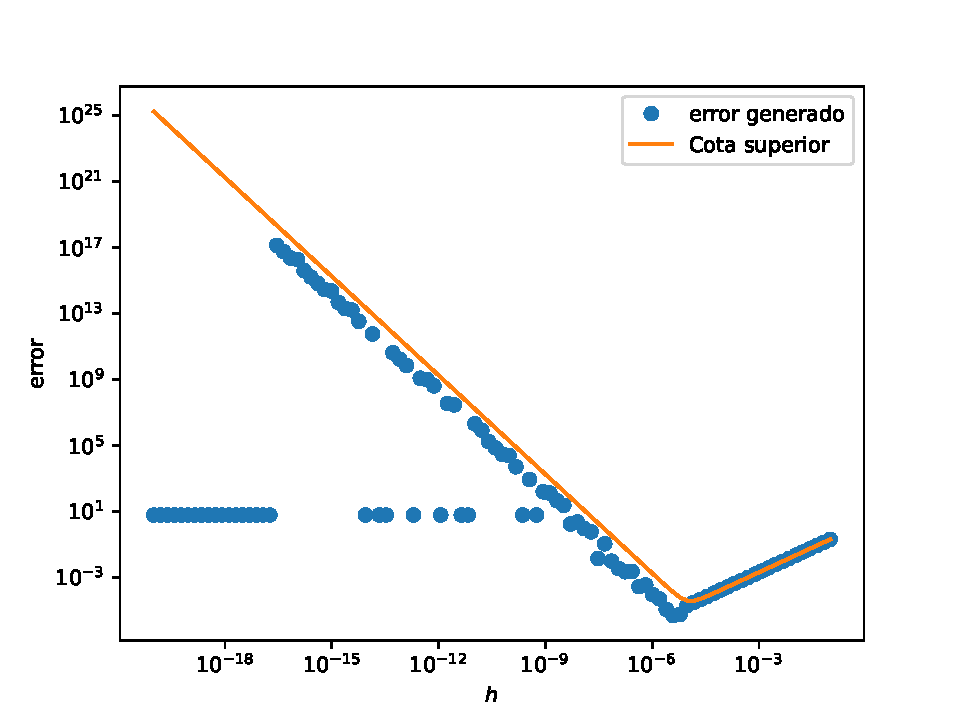
\includegraphics[width=0.5\linewidth]{contenido/img/graficodeerrorcontrol1.pdf}
    \caption{Error real y cota superior del error en la función $f(x)=x^3$}
    \label{fig:errorcontrol1}
\end{figure}
Como se aprecia en el grafico $(h,E(h))$, la cota superior del error funciona correctamente (fig \ref{fig:errorcontrol1})

\include{}
\include{}
\include{}
\include{}
\include{}
\include{}


% Conclusiones y referencias
\documentclass[../portafolio.tex]{subfiles}

\begin{document}

\chapter*{Conclusiones}
\addcontentsline{toc}{chapter}{Conclusiones}
\markboth{Conclusiones}{Conclusiones}

\hfill \textbf{Fecha de presentación:} Viernes 29 de noviembre de 2024

\medskip

% ESTE CAPÍTULO LO DEBES LLENAR AL FINALIZAR LA ASIGNATURA, por supuesto antes de la fecha de entrega.

%--------------------------------------------------------------------------------
% Inicie con un resumen breve de cuáles eran los objetivos del portafolio;

%--------------------------------------------------------------------------------
% [Resumen de los contenidos]
% - Un resumen MUY breve de cuáles son las evidencias de aprendizaje que incluyó en este portafolio. Algo como "En el capítulo 1, se derivó numéricamente la función coseno, usando un esquema de derivadas centradas, para estudiar el error absoluto con respecto a la derivada analítica de la misma función."
% - Incluya una breve reflexión de lo que aprendió en cada actividad, lo que faltó aprender, lo que no se entendió y lo que sí se entendió bien.
% - Haga lo anterior por cada evidencia de aprendizaje.


%--------------------------------------------------------------------------------
% [Autoevaluación del alumno/a]
% Realice una reflexión de cómo trabajó usted, qué cree haber hecho bien y mal en el curso, qué le gustaría  hacer a futuro (en la forma de estudiar y en cómo cree que aplicará los contenidos de este portafolio en el futuro), cómo han distribuido su trabajo a lo largo del trabajo en este portafolio.

% --------------------------------------------------------------------------------
% [Evaluación del curso]
% - Realice una comparación entre sus expectativas iniciales, tal como las describió en la sección de presentación, y lo que realmente aprendió y experimentó a lo largo del curso. ¿Se cumplieron sus expectativas sobre la asignatura? ¿En qué medida?
% - ¿Qué aspectos del curso o del portafolio superaron, igualaron o no alcanzaron sus expectativas iniciales?
% - Agregue sugerencias para futuras versiones del curso, para que estudiantes de generaciones venideras se beneficien de una aplicación mejorada de este instrumento de evaluación.
% - ¿Cuál es la evidencia de este portafolio que usted cree es mejor/más relevante/en la que aprendió mejor? ¿Qué diferencia a esa evidencia del resto incluido en este portafolio?
% - ¿Puede evaluar la utilidad de este portafolio?


\end{document}


%%%%%%%%%%%%%%%%%%%%%%%%%%%%%%%%%%%%%%%%%%%%%%%%%%%%%%%%%%%%%%%%%%%%%%
% Puede usar el capítulo de apéndice para agregar sus códigos completos si lo desea
% \appendix
% \subfile{tex/...}

% lista de referencias guardadas en referencias.bib
\bibliography{referencias}

\end{document}